		\chapter{Laser Localization System}
        	\label{laser_localization}
            \index{laser}
            \index{laser localization}
			This was one of the unfortunate systems that were cut in liue of lack of time. I have a large wheeled base which I was going to incorporate into the \index{routine}routine - however unfortunately it doesn't have the best dead-reckoning ability (one wheel turns significantly faster than the other).\\
			
			Whilst this can be fixed using speed ratios in code, I didn't feel it would be accurate enough for the purposes.\\
			
			Of course, another solution would be to use rotary encoders, however the resources and opportunity for me to install them didn't present themselves.\\
			
			As I was intending on using the system in \index{regionals}Regionals, I developed this cheap, quick, easy, and accurate way of localizing a robot in the dance area using equipment and sensors that I already had, along with <\$50 of parts.\\
			
			I was ready to build this system - I had the parts, the maths, parts of the code, and the concept ready to go - I just lacked the time to actually put it together!
			
			I originally \href{http://goo.gl/u1BwKA}{\textit{posted a question}} asking the feasibility of said system on the Parallax Forums, and got lots of interesting thoughts to help with this idea.
			
			It's possibly also worth mentioning that I had designed a completely different system based on IR, but decided not to use it. For the sake of brevity, I'll exclude going into detail about it.
			
			\section{System Concepts}
				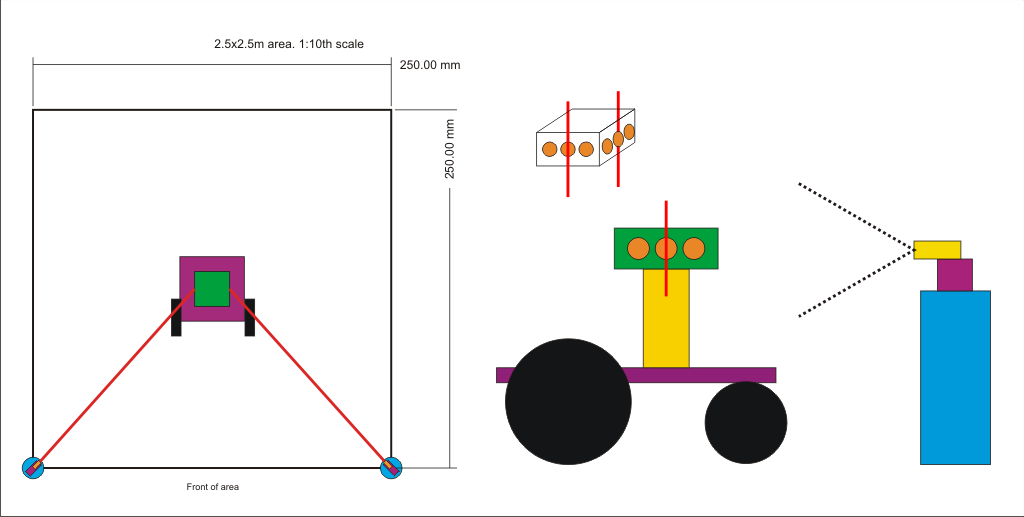
\includegraphics[width=\linewidth]{images/laser_localization_system}
				
				In the figure above, the outer 2.5m area is the bounds of where the robot is allowed to go. The system will not have to track outside this area. The big purple square is the robotic base I'm trying to track, there are two black wheels either side of it. Now focus your attention to the circles on the bottom left and bottom right of the 2.5m area. The purple squares at 45d are servo motors. The gold squares mounted on top of the servos are line lasers (with the lines set vertically).\\
				
				Now focus your attention to the diagram to the right of the square area, you can see a side on view of the robot base. The yellow block on the robot is simply a wooden spacer. The green box on top of that is a "cube" of circuit boards, with 3 \index{LDR}\index{phototransistor}\index{photodiode}LDRs/Phototransistors/Photodiodes on each side (denoted by orange circles). (See figure above the side on robot view for a 3D representation). To the right of the side on view of the robot is the \index{beacon}"beacon/laser scanner". The blue denotes a wooden block, purple denotes servo, gold denotes line laser.\\
				
				\textbf{\textit{NOTE: }}At this time I wasn't aware I had some TAOS linescan sensors in my possession, so I was still working with the concept of using LDRs. Since then I updated the idea to work using said TAOS linescan sensors. The advantages of the Linescan sensors were clear - faster response times and wider sensing areas.
				
				\centerline{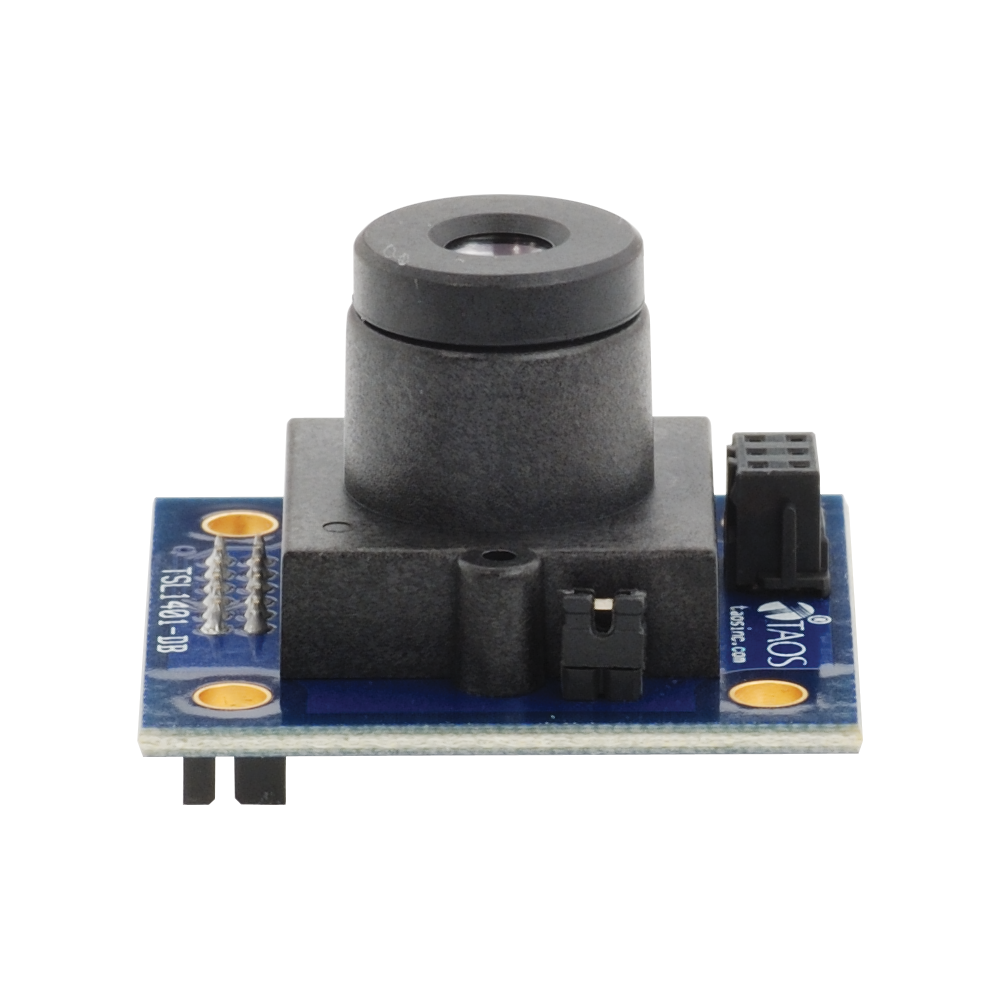
\includegraphics[width=0.5\linewidth]{images/linescan_sensor}}
				
			\section{Laser Tracking}		
				When the system first turns on, the servo (and thus the laser) scans throughout it's range. When the middle LDR on the robot detects the laser, it sends a message over an RF link to the beacon. The laser should be focused on the centre LDR. (as the diagrams denote). Please remember that I've updated this idea to work using TAOS \index{linescan}\index{sensors}Linescan sensors instead of LDRs.
				
				The second laser will do the same, although will be focusing it's laser on a different side of the "LDR cube". (since updated this to, the laser will be focused at a different section of the linescan sensor's sensing area). At this point in time the system knows the position of each beacon, along with the angle from each beacon to the robot. It will then \index{bilateration}bilaterate the position of the robot.
				
			\section{Issues with the LDR System}
				As I've amply mentioned, I resigned the system to use TAOS linescan sensors instead of the LDRs for a few reasons, mainly because of limited sensing area, and speed.\\
				
				Here's an excerpt of the forum post outlining my concerns:\\
				
				\textit{I'm wanting the robot to move 0.5m-1m / second. That equates to 0.5mm-1mm / millisecond. The LDRs I'm wanting to use have a size of ~8mm\^2. That means there's a distance of 12mm from the centre of the middle LDR to either outside edge (where it looses detection). That means, in perfect conditions, you'd have ~8ms between the time that the robot starts moving at 1m/s, and when the laser moves off the edge LDR. Thus, the loop between the laser hitting the outer LDR, sending the signal to the beacon, the beacon processing that and moving has to be under 8ms (at the very most). For reference I'm currently using the \index{nRF24L01+}\hyperref[sec:nRF24L01+]{nRF24L01+} transceiver modules, which had a response time of <2ms when I tested them (in unoptimized conditions).}
				
				My current testing with the TAOS sensors have been promising, but I haven't tested the system in it's entirety. 
							
			\section{Rule Legality \& Safety Considerations}
            	\index{safety}
				Understandably there are some concerns with using lasers where there are lots of humans around, and the hazards associated with it shining in their eyes.\\
				
				I approached Mr. Jason Bell, and Dr. Damien Kee with my concerns, seeking clarity. The answer I received was that I should be able to, provided the lasers meet Australian Standards.\\
				
				As such, I set out to seek whether the lasers I was intending to use meet such criteria. Here's an email I composed to Mr. Jason Bell, and Dr. Damien Kee outlining my research and conclusions on said topics.\\
				
				\pagebreak
                
				
				\begin{quote}
					{\itshape
					Hi Dr. Kee,\\
						
					Following our recent discussion about using lasers in RCJA Dance, I can offer the following comments about the lasers I'm wanting to use:\\
					
					The Weapons Act defines a Laser Pointer as a hand-held battery-operated device, with a power output of more than 1 milliwatt, that is designed to emit a laser beam and may be used for aiming, pointing or targeting.\\
                    
					My laser uses 5mW, but does not concentrate that energy to a single point, but rather spreads it out over a line, reducing the concentration of the beam. I rang up the Weapons Department of the Government to seek clarity in this matter, and ensure that it'd be safe enough for the competition. They have indicated that this type of laser fell outside the reasonable definition of a "Laser Pointer" under the Weapons Act.\\
					
					Finally, all due care and attention will be given to using the lasers in a safe and responsible way, and the issues will be dealt with in the following ways: The line laser will be pulsed on for the minimum required time to take a reading, which is around 50ms (reducing it's overall power). The line laser is mounted within a protective covering, reducing stray laser light, and facing away from the audience at all times.\\
					
					I am satisfied that if used safely, this type of line laser falls within the guidelines of the competition, but I would like your final consideration before proceeding. I don't imagine I'll have enough time before the competition to actually assemble this system, but in the off chance I do I would appreciate your go-ahead.\\
					
					Kind Regards,\\					
					John Board}
				\end{quote}	
				\pagebreak
				
				The response to the letter was positive, and the final ruling was that such system was allowed at a Regional level.